\documentclass[11pt,a4paper]{report}
\usepackage{amsmath,amsfonts,amssymb,amsthm,epsfig,epstopdf,titling,url,array}
\usepackage{enumitem}
\usepackage{changepage}
\usepackage{graphicx}
\usepackage{caption}
\theoremstyle{plain}
\newtheorem{thm}{Theorem}[section]
\newtheorem{lem}[thm]{Lemma}
\newtheorem{prop}[thm]{Proposition}
\newtheorem*{cor}{Corollary}
\theoremstyle{definition}
\newtheorem{defn}{Definition}[section]
\newtheorem{conj}{Conjecture}[section]
\newtheorem{exmp}{Example}[section]
\newtheorem{exercise}{Exercise}[section]
\theoremstyle{remark}
\newtheorem*{rem}{Remark}
\newtheorem*{note}{Note}
\def\changemargin#1#2{\list{}{\rightmargin#2\leftmargin#1}\item[]}
\let\endchangemargin=\endlist 
\begin{document}


\section*{Problem}
\begin{enumerate}[label=(\alph*)]
\item {Suppose that in the picture below, the triangle is equilateral and the circle has radius 1. Find the length of a side of the triangle.
\begin{figure}[h!]
  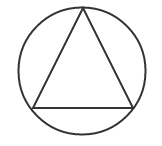
\includegraphics[width=2in]{triangle.png}
  {\caption*{}}
  \label{}
\end{figure}}
\end{enumerate}
\section*{Bonus}
\begin{enumerate}[label=(\alph*)]\addtocounter{enumi}{1}
\item Generalize your solution to derive a formula
for $s(n)$ = the length of a side of an 
$n$-sided regular polygon inscribed in the unit circle.
\item Find $lim_{n\to\infty}s(n)$
\item Find $lim_{n\to\infty}p(n) = ns(n)$
\item Explain why the limits in parts $c$ and $d$ 
 make sense.
\end{enumerate}

\newpage
\section*{Solution (part a)}
Rotate the original diagram clockwise by $\pi/2$ radians and set up
a coordinate system as shown in the picture below.

\begin{figure}[h!]
  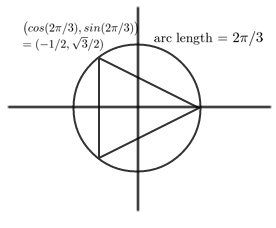
\includegraphics[width=3in]{triangle2.png}
  {\caption*{}}
  \label{}
\end{figure}

Since all angles of the triangle are the same, the arc length of each of
the three arcs that the triangle cuts the unit circle into is $2\pi/3$. So the coordinates of the vertex in the second quadrant must be
$\big(cos(2\pi/3), sin(2\pi/3)\big)$ or $(-1/2,\sqrt{3}/2).$  We can find the length of the side from the vertex on the $x$ axis to this point using the distance formula:
$$\sqrt{(-1/2 - 1)^2 + (\sqrt{3}/2 - 0)^2} = \sqrt{3}$$

\section*{(part b)}
Using the same argument as in part a), an $n$-sided polygon will cut the circle into $n$ arcs, each of size $2\pi/n$ radians.  The side along the first arc moving counter-clockwise along the unit circle from the $x$-axis will have the following length, again using the distance formula:
$$s(n) = \sqrt{(cos(2\pi/n) - 1)^2 + (sin(2\pi/n) - 0)^2}$$

\section*{(part c)}
As $n \to \infty$, $cos(2\pi/n) \to cos(0) = 1$ and $sin(2\pi/n) \to sin(0) = 0$, so $s(n) \to \sqrt{ (1 - 1)^2 - (0 - 0)^2} = 0$.

\section*{(part d)}
This one is a little trickier.  Note that $p(n)$ is the perimeter of the inscribed polygon.  Intuitively, this should converge on the circumference of the circle, which is $2\pi$.  Of course, mathematics does not fail us here.
$$lim_{n\to\infty}p(n) = $$
$$lim_{n\to\infty} n\sqrt{(cos(2\pi/n) - 1)^2 + (sin(2\pi/n) - 0)^2} = $$
OK, this is sneaky (move $n$ under the radical and multiply and divide by $2\pi$)
$$lim_{n\to\infty}2\pi\sqrt{\frac{n^2(cos(2\pi/n) - 1)^2 + n^2(sin(2\pi/n))^2}{ (2\pi)^2}} = $$
$$lim_{n\to\infty}2\pi\sqrt{\frac{n^2(cos(2\pi/n) - 1)^2}{(2\pi)^2} + \frac{n^2(sin(2\pi/n))^2}{(2\pi)^2}} = $$
$$lim_{n\to\infty}2\pi\sqrt{\frac{(cos(2\pi/n) - 1)^2}{(2\pi/n)^2} + \frac{(sin(2\pi/n))^2}{(2\pi/n)^2}} = $$
$$ lim_{n\to\infty}2\pi\sqrt{\Big(\frac{(cos(2\pi/n) - 1)}{(2\pi/n)}\Big)^2 + \Big(\frac{(sin(2\pi/n))}{(2\pi/n)}\Big)^2}.$$

Now, by L'Hospital's rule (see below), $\lim_{x\to 0}\frac{cos(x) - 1}{x} = \lim_{x\to 0}\frac{-sin(x)}{1} = 0$ and $\lim_{x\to 0}sin(x)/x = \lim_{x\to 0}cos(x)/1 = 1$. As ${n\to\infty}$, $2\pi/n\to 0$, so the quantity under the radical in the last expression above approaches $0^2 + 1^2 = 1$.  That makes the entire limit equal to $2\pi$.  

\section*{(part e)}
As $n \to \infty$, the inscribed polygon approaches the circle, so as noted in the solution to d), it makes sense that its perimeter approaches the circumference of the circle.  The length, $s(n)$, of a single side has to go to $0$ because the sides all have the same length and for each $n$, $p(n) = ns(n)$ is finite, actually bounded above by $2\pi$ (another nice exercise to prove - hint: shortest distance between two points is a straight line).

\pagebreak
\section*{L'Hospital's Rule}
The form of L'Hospital's rule that we use above is this: \\\\
Suppose that $f$ and $g$ are continuously differentiable throughout an open interval containing the point $c$ in its interior.  Suppose further that $f(c) = g(c) = 0$ and that $\mathop{\lim}\limits_{x\to c}\frac{f'(x)}{g'(x)}$ exists.  Then 
$$\mathop{\lim}\limits_{x\to c}\frac{f(x)}{g(x)} = \mathop{\lim}\limits_{x\to c}\frac{f'(x)}{g'(x)}$$
The proof of this form of the rule follows directly from the definition of the derivative:
Recall that the derivative of $f$ at $x$ is defined by
$$f'(x) = \lim_{h \to 0} \frac{f(x + h) - f(x)}{h}.$$
So $$\frac{f'(c)}{g'(c)} = $$
$$\frac{\mathop{\lim}\limits_{h \to 0} \frac {f(c + h) - f(c)} {h}} {\mathop{\lim}\limits_{h \to 0} \frac {g(c + h) - g(c)} {h}} = $$
$$\lim_{h \to 0} \frac {f(c + h) - f(c)} {g(c + h) - g(c)} = $$
$$\lim_{h \to 0} \frac {f(c + h)} {g(c + h)} = $$
$$\lim_{x \to c} \frac {f(x)} {g(x)}.$$ 
Now since our assumption is that $f'$ and $g'$ are continuous, it follows that 
$$\mathop{\lim}\limits_{x\to c}\frac{f'(x)}{g'(x)} = \frac{f'(c)}{g'(c)}$$,so we have shown that 
$$\mathop{\lim}\limits_{x\to c}\frac{f(x)}{g(x)} = \mathop{\lim}\limits_{x\to c}\frac{f'(x)}{g'(x)}.$$$$\lim_{h \to 0} \frac {f(c + h)} {g(c + h)} 
\end{document}

